\documentclass[11pt]{article}
\usepackage[T1]{fontenc}
\usepackage[utf8]{inputenc}
\usepackage{lmodern,microtype,amsmath,amssymb,amsthm,mathtools,mathrsfs}
\usepackage[margin=30mm]{geometry}
\usepackage{booktabs,enumitem,tikz,xcolor,xurl}
\usetikzlibrary{arrows.meta,positioning,calc}
\usepackage[unicode,colorlinks=true,linkcolor=blue!45!black,urlcolor=blue!55!black,citecolor=green!35!black]{hyperref}
\setlength{\emergencystretch}{2em}
\numberwithin{equation}{section}
\newtheorem{theorem}{Theorem}[section]
\newtheorem{proposition}[theorem]{Proposition}
\newtheorem{lemma}[theorem]{Lemma}
\newtheorem{corollary}[theorem]{Corollary}
\theoremstyle{definition}\newtheorem{definition}[theorem]{Definition}
\theoremstyle{remark}\newtheorem{remark}[theorem]{Remark}
\newcommand{\ii}{\mathrm i}\newcommand{\dd}{\mathrm d}
\newcommand{\CC}{\mathbb C}\newcommand{\RR}{\mathbb R}\newcommand{\ZZ}{\mathbb Z}
\newcommand{\cH}{\mathcal H}\newcommand{\Bhat}{\widehat B}
\newcommand{\Turn}{\mathsf T}\newcommand{\Cheb}{\mathsf C}
\newcommand{\Tr}{\operatorname{Tr}}\newcommand{\arccot}{\operatorname{arccot}}
\newcommand{\T}{\mathsf T}\newcommand{\HH}{\mathcal H}\newcommand{\A}{\mathcal A}
\newcommand{\eps}{\varepsilon}
\title{Newton calculus and stationary profiles of Conway tangles}
\author{}\date{}
\begin{document}\maketitle
\begin{abstract}
At a principal root of unity, the two-strand Casimir has repeated
spectral roots. We construct its full Newton calculus, including
multiplication, physical quarter-turn, marked closure and colored
crossing circles, with the derivative data at repeated roots retained.
For arbitrary ordered Conway expressions, we determine the exact
positive integer support and characterize the existence of a strict
real state. For every expression admitting a strict state, the complete
positive source has a unique interior maximum
with negative definite Hessian on its primitive wire lattice. Its
logarithmic growth equals this maximum at both level parities.
We calculate stationary boundary profiles with their additive constants
and prove an exact harmonic response law. Every original leaf at a
closed strict maximum lies at or above one quarter; a specified
completed-root subclass satisfies stronger bounds. The positive source
studied here provides finite and variational input for separate estimates
of signed fillings and their hyperbolic volumes.
\end{abstract}

\section{Introduction}
A tangle calculation changes character when two spectral roots
coincide. Polynomial values alone no longer determine the operator:
a derivative can multiply a nonzero nilpotent matrix. This paper uses
one polynomial algebra throughout the tangle calculation, keeping both
values and first derivatives. Its basis is chosen so that the physical
quarter-turn reverses the basis index. Multiplication then has positive
coefficients with a simple support, and cylindrical closure pairs
complementary indices.

These identities turn any fixed ordered expression in two-strand
tangles into a finite sum over integer indices. For the complete color
on every auxiliary circle, every nonzero summand is positive. The
positivity makes a variational question natural: which expressions
have an interior maximizing state, and how does that state respond
when the exposed output index changes?

The exact finite calculus is proved in
Proposition~\ref{prop:newton-turn}, Theorem~\ref{thm:positive-product}
and Proposition~\ref{prop:circle}. The strict support criterion is
Theorem~\ref{st:reduced-junctions}. Theorem~\ref{st:positive-action}
proves the unique interior maximum, its nondegenerate Hessian and the
positive-source limit. Its boundary argument is necessary: concavity
by itself would permit a maximum on the boundary. Theorems
\ref{st:profiles} and \ref{st:probe} calculate the absolute stationary
profiles. Theorem~\ref{st:quarter} and Lemma~\ref{lem:port-bounds}
give respectively the general and completed-root leaf bounds.

All expressions and their number of leaves are fixed before the
quantum level grows. No tangle-isotopy classification is needed.
The positive auxiliary source still has to be compared with signed
terms and with the entire filling sum before it supplies a volume
limit for an invariant.

Kashaev's crossing-matrix definition supplies the knot-theoretic
background \cite{Kashaev1995}. The exact enhanced normalization used
here is compared with that definition, for $N\ge3$, in
\cite[Theorem~10.1]{Finite}. The finite identities below also hold
at $N=2$. Rational-tangle conventions are discussed in
\cite{KauffmanLambropoulou}; we fix the ordered endpoints explicitly.
The angle-variable concavity used in our variational proof is discussed
in the Casson--Rivin exposition \cite{FuterGueritaud}. Here the
polytope, integer approximation and boundary proof are established
directly. A global hyperbolic metric is a separate construction.

\section{The diagrams and the positive source}\label{nt:diagrams}
A two-string tangle consists of two arcs in a ball with four prescribed
boundary points. Additional closed curves are allowed and will include
the auxiliary crossing circles. Label the exposed endpoints in their
cyclic order by
\[
0=\text{bottom left},\quad1=\text{bottom right},\quad
2=\text{top right},\quad3=\text{top left}.
\]
For a vertical stack $FG$, place $F$ below $G$ and join $F_2$ to $G_1$
and $F_3$ to $G_0$. The exposed tuple is $(F_0,F_1,G_2,G_3)$.
A clockwise quarter-turn carries the entire tangle with its box; the
new tuple is $(F_1,F_2,F_3,F_0)$ in terms of the old labels.
Cylindrical closure $C(FG)$ joins the remaining bottom and top endpoints
on each side, without additional crossings. These connections are shown
in Figure~\ref{nt:operations}.

\begin{figure}[ht]
\centering% Ordered boundary connections; boxes suppress their interior tangles.
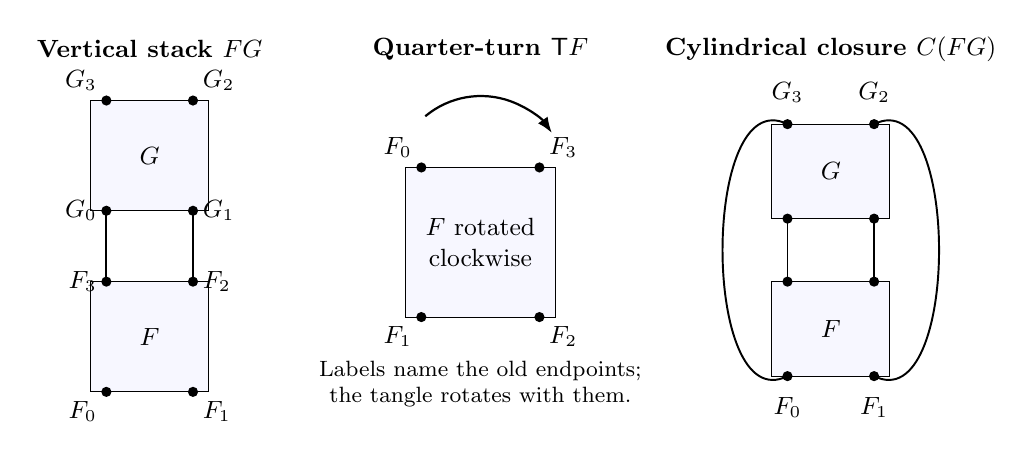
\begin{tikzpicture}[x=1cm,y=1cm, every node/.style={font=\small},
 tangent/.style={line width=.7pt}, terminal/.style={circle,fill=black,inner sep=1.3pt}]
% Left: stacking.
\begin{scope}[shift={(0,0)}]
 \node[font=\small\bfseries] at (1.2,4.8) {Vertical stack $FG$};
 \draw[fill=blue!3] (.45,.45) rectangle (1.95,1.85);
 \draw[fill=blue!3] (.45,2.75) rectangle (1.95,4.15);
 \node at (1.2,1.15) {$F$}; \node at (1.2,3.45) {$G$};
 \foreach \x in {.65,1.75} {
  \draw[tangent] (\x,1.85)--(\x,2.75);
  \foreach \y in {.45,1.85,2.75,4.15} \node[terminal] at (\x,\y) {};
 }
 \node[below left] at (.65,.45) {$F_0$};\node[below right] at (1.75,.45) {$F_1$};
 \node[left] at (.65,1.85) {$F_3$};\node[right] at (1.75,1.85) {$F_2$};
 \node[left] at (.65,2.75) {$G_0$};\node[right] at (1.75,2.75) {$G_1$};
 \node[above left] at (.65,4.15) {$G_3$};\node[above right] at (1.75,4.15) {$G_2$};
\end{scope}
% Middle: a genuine clockwise turn, showing old labels in new positions.
\begin{scope}[shift={(4.25,0)}]
 \node[font=\small\bfseries] at (1.15,4.8) {Quarter-turn $\mathsf T F$};
 \draw[fill=blue!3] (.2,1.4) rectangle (2.1,3.3);
 \node[align=center] at (1.15,2.35) {$F$ rotated\\clockwise};
 \foreach \p in {(.4,1.4),(1.9,1.4),(1.9,3.3),(.4,3.3)} \node[terminal] at \p {};
 \node[below left] at (.4,1.4) {$F_1$};\node[below right] at (1.9,1.4) {$F_2$};
 \node[above right] at (1.9,3.3) {$F_3$};\node[above left] at (.4,3.3) {$F_0$};
 \draw[-{Latex[length=2mm]},thick] (.45,3.95) arc[start angle=130,end angle=35,radius=1.1];
 \node[align=center,font=\footnotesize] at (1.15,.55) {Labels name the old endpoints;\\the tangle rotates with them.};
\end{scope}
% Right: closure arcs are actual identity connections outside both boxes.
\begin{scope}[shift={(8.65,0)}]
 \node[font=\small\bfseries] at (1.2,4.8) {Cylindrical closure $C(FG)$};
 \draw[fill=blue!3] (.45,.65) rectangle (1.95,1.85);
 \draw[fill=blue!3] (.45,2.65) rectangle (1.95,3.85);
 \node at (1.2,1.25) {$F$};\node at (1.2,3.25) {$G$};
 \foreach \x in {.65,1.75} {
  \draw[tangent] (\x,1.85)--(\x,2.65);
  \foreach \y in {.65,1.85,2.65,3.85} \node[terminal] at (\x,\y) {};
 }
 \draw[tangent] (.65,.65)..controls(-.45,.1)and(-.45,4.4)..(.65,3.85);
 \draw[tangent] (1.75,.65)..controls(2.85,.1)and(2.85,4.4)..(1.75,3.85);
 \node[below] at (.65,.5) {$F_0$};\node[below] at (1.75,.5) {$F_1$};
 \node[above] at (.65,4.0) {$G_3$};\node[above] at (1.75,4.0) {$G_2$};
\end{scope}
\end{tikzpicture}

\caption{Stacking, clockwise rotation and cylindrical closure. Each box
contains its entire tangle. The outside arcs specify the actual
connections used in the evaluation.}\label{nt:operations}
\end{figure}

Let $L_j$ be an auxiliary circle carrying the $j$-dimensional
highest-weight representation and surrounding two main strands of
complete color $N$. Its disk fixes the ordering and framing. Set
$h_j=\Turn L_j$. When discussing the construction, $h$ denotes one
such turned circle; in the positive source it is evaluated as $h_N$.
Every written occurrence is a distinct auxiliary circle.

The open expressions considered here have arbitrary ordered syntax
\[
 E::=h\mid\Turn E\mid E_1E_2.
\]
A closed expression is $C(FG)$. Every written occurrence of $h$ is a
distinct auxiliary circle. The complete positive source $Z_N^0$ is
its evaluation with every leaf equal to $h_N$ and no retained half
twists. Section~\ref{nt:algebra} defines this scalar as $\phi(FG)$.
Its endpoint pairing need not form a knot; that condition belongs
to later knot applications. For example, $C((hh)(hh))$ has four
leaves and $C(h\Turn(hh))$ has three. Section~\ref{nt:completed}
will distinguish a narrower recursive class with stronger bounds.

\section{The physical pair algebra}\label{nt:algebra}
Fix $N\ge2$, and set
\begin{equation}\label{eq:root-notation}
 d=N-1,\qquad q=e^{\pi\ii/N},\qquad Q=q^2,\qquad
 x=q^d,\qquad \kappa=q^{d^2/2},\qquad \rho=q-q^{-1}.
\end{equation}
There is no restriction to prime or odd $N$. The main strands carry the $N$-dimensional vector space $V_N$; this is what ``complete color'' means at this stage. The operators $H,K,E,F$ encode its quantum-group action. They are concrete matrices, which we specify so that the crossing convention can be checked. One convenient choice of basis is $v_0,\ldots,v_d$ and
\[
 H v_j=(d-2j)v_j,\quad K=q^H,\quad
 E v_j=[j]_q^2v_{j-1},\quad Fv_j=v_{j+1},
 \qquad [j]_q=\frac{q^j-q^{-j}}{q-q^{-1}}.
\]
Missing endpoint vectors are zero. For $k\ge0$, the quantum factorial is
$[k]_q!=\prod_{r=1}^k[r]_q$, with $[0]_q!=1$.
The finite universal crossing, including its Cartan factor, is
\begin{equation}\label{eq:universal-crossing}
 \mathscr R=q^{H\otimes H/2}
 \sum_{k=0}^{d}\frac{q^{k(k-1)/2}\rho^k}{[k]_q!}
 E^k\otimes F^k.
\end{equation}
Every denominator is nonzero. The physical braided crossing is obtained with the fixed exchange and transpose convention; the inverse is the actual matrix inverse. The framing and enhancement are part of the definition, not an unspecified factor appended to an asymptotic formula.

For calculations in the polynomial algebra it is useful to change basis on this same space. We call the new coordinates balanced; they do not define a different invariant. In this basis the operators are
\begin{equation}\label{eq:balanced-module}
 \mathcal E|a\rangle=(Q^{-a}-1)|a-1\rangle,\quad
 \mathcal F|a\rangle=(1-Q^{a+1})|a+1\rangle,\quad
 K|a\rangle=xQ^{-a}|a\rangle.
\end{equation}
The ordinary cup and cap, and the one marked cap, have entries
\begin{equation}\label{eq:cups}
 p_{ab}=Nx^{-b}\delta_{a+b,d},\qquad
 \ell_{ab}=\frac{x^a}{N}\delta_{a+b,d},\qquad
 m_{ab}=\frac{x^b}{N^2}.
\end{equation}
The cup creates two endpoints and the cap joins them. Their two snake identities say that a bend followed by the opposite bend evaluates to a straight strand. The different marked cap implements the reduced invariant and satisfies $mp=1$. The diagonal operator $g=K^{1-N}=(-1)^dK$ is the \emph{pivot}, the correction inserted when an ordinary strand is closed by a trace. For a two-strand operator $A$ commuting with the pair quantum-group action, the original cylindrical evaluation is
\begin{equation}\label{eq:phi-physical}
 \phi(A)=\frac1N\Tr_{V_N\otimes V_N}\bigl[(I\otimes g)A\bigr].
\end{equation}
The factor $1/N$ in this expression is the single cut average. It is not repeated at the auxiliary circles.


In the ordinary highest-weight basis above, put
$p_a=\prod_{j=1}^a(1-Q^j)$. The balanced basis is
$|a\rangle=\rho^a p_a^{-1}v_a$, with
$\mathcal E=\rho E$ and $\mathcal F=\rho F$.
All $p_a$ with $a<N$ are nonzero. This gives an explicit diagonal
change of basis on the same representation. Its factors cancel on
contracted wires. The invariant normalization and crossing comparison
are those of \cite[Theorem~10.1]{Finite}; no asymptotic bound on this
change of basis is used.

\subsection{The full pair algebra}

An operator on two strands must commute with the joint action of the quantum-group generators if it is to represent one of our invariant tangle boxes. The formulas below specify that joint action. The subsequent lemma identifies all such commuting operators; this is the meaning of the term \emph{commutant}.
The balanced pair generators and Casimir are
\begin{equation}\label{eq:pair-casimir}
 \mathcal E_{12}=\mathcal E_1K_2+\mathcal E_2,\quad
 \mathcal F_{12}=\mathcal F_1+K_1^{-1}\mathcal F_2,\quad
 K_{12}=K_1K_2,\quad
 \Omega=\mathcal F_{12}\mathcal E_{12}+qK_{12}+q^{-1}K_{12}^{-1}.
\end{equation}
Let $\Cheb_n(z)=2T_n(z/2)$, where $T_n$ is the usual Chebyshev polynomial. Thus $\Cheb_0=2$, $\Cheb_1=z$ and $\Cheb_{n+1}=z\Cheb_n-\Cheb_{n-1}$. Define
\begin{equation}\label{eq:hermite-algebra}
 P_N(z)=\Cheb_N(z)+2=\prod_{j=0}^{d}(z-c_j),\qquad
 c_j=q^{2j+1}+q^{-2j-1},\qquad
 \cH_N=\CC[z]/(P_N).
\end{equation}
The list of roots includes multiplicity. Since $c_{d-j}=c_j$, all distinct roots are double except the simple root $-2$ at odd $N$.

\begin{lemma}[Full commutant]\label{lem:commutant}
The endomorphisms of $V_N\otimes V_N$ commuting with the three pair generators are exactly $\CC[\Omega]\simeq\cH_N$.
\end{lemma}
\begin{proof}
Let $W_T$ be the span of $|a,T-a\rangle$. The $K_{12}$ eigenvalue one occurs only on $W_d$. The matrices $\mathcal E_{12}:W_{T+1}\to W_T$ for $T<d$, and $\mathcal F_{12}:W_T\to W_{T+1}$ for $T\ge d$, have triangular maximal minors with nonzero diagonals. Consequently the entire pair is generated from $W_d$ by these raising and lowering operators.

On $W_d$, the Casimir is a symmetric tridiagonal matrix with adjacent entries $-(1-Q^{a+1})^2\ne0$. Its first basis vector is cyclic: the $k$th power has last possible coordinate $k$, with coefficient equal to the nonzero product of the first $k$ adjacent entries. An operator commuting with this block is therefore a unique polynomial of degree below $N$ in that block. Subtracting the same polynomial in $\Omega$ from a pair intertwiner gives zero on $W_d$, hence zero everywhere by generation.

Before specialization, use a variable $\zeta$ and the ordinary
highest-weight module of highest weight $d$, with weights $d-2a$,
$E v_a=[a]_\zeta[N-a]_\zeta v_{a-1}$ and $Fv_a=v_{a+1}$.
At the principal root $[N-a]_q=[a]_q$, so this specializes to the
module already defined. The balanced diagonal change is regular there. In the pair, a highest vector of total degree $j$ is obtained by solving the bidiagonal raising equation. If its coefficient at $|a,j-a\rangle$ is $u_a$, the equation at $|a,j-a-1\rangle$ determines $u_{a+1}/u_a$ as the negative ratio of the two nonzero raising entries. Thus for generic $q$ there is one such vector in each degree $j=0,\ldots,d$. Its highest weight is $2d-2j$, its Casimir is $q^{2d-2j+1}+q^{-2d+2j-1}$, and its successive lowering vectors are nonzero through the usual length. The dimensions $2d-2j+1$ sum to $N^2$. Distinct generic Casimirs make these submodules independent.

In degree $T\le d$, precisely the highest vectors $j\le T$ contribute one descendant each. Their eigenvalues give the block characteristic polynomial. At $q=e^{\pi\ii/N}$ it becomes
\[
 \prod_{j=0}^{T}(z-c_j),\qquad c_j=q^{2j+1}+q^{-2j-1}.
\]
All physical matrix entries specialize regularly. The nonzero adjacent entries of the tridiagonal block make a boundary vector cyclic, so this characteristic polynomial is also minimal even when roots coincide. At $T=d$ it is $P_N$. The elementary identity
\[
 \prod_{j=0}^{N-1}(z-q^{2j+1}-q^{-2j-1})=2T_N(z/2)+2
\]
can also be checked by putting $z=w+w^{-1}$: the roots correspond to $w^N=-1$, and the monic degree and leading coefficient agree. The generating property of $W_d$ propagates its vanishing to the full pair.


This proves the polynomial relation and the full commutant assertion.

\end{proof}

At a double root $c$, reduction modulo $(z-c)^2$ leaves
\[
 f(z)=f(c)+f'(c)(z-c)\pmod{(z-c)^2}.
\]
Thus both the value and its first derivative are independent coordinates of the operator. Throughout the paper, retaining the ``full algebra'' or the ``normal data'' means retaining this derivative as well. A polynomial can vanish at every distinct root and still define a nonzero operator in $\cH_N$. Evaluating only at roots would therefore lose part of the invariant.

\subsection{The actual turn and the Newton basis}

We choose a polynomial basis adapted to successive Casimir roots, including their multiplicities. Its normalization is designed so that turning a physical box reverses the basis index exactly. The same basis makes the final closure a coefficient extraction. These are the two facts that will allow us to follow every internal summation index through a large construction.
Put
\begin{equation}\label{eq:newton-basis}
 s_r=\prod_{u=1}^{r}2\sin\frac{\pi u}{N},\quad s_0=1,\qquad
 B_r(z)=\prod_{j=0}^{r-1}(c_j-z),\qquad
 \Bhat_r(z)=\frac{B_r(z)}{s_r^2},\quad 0\le r\le d.
\end{equation}
The quarter-turn is the literal contraction
\[
 \Turn(A)=(I^{\otimes2}\otimes\ell)(I\otimes A\otimes I)
 (p\otimes I^{\otimes2}).
\]
Its entries in the recorded all-primal chart are
\[
 \Turn(A)_{(a,b);(c,e)}=x^{a-e}A_{(b,d-e);(d-a,c)}.
\]
The cups and caps are those of \eqref{eq:cups}. Direct substitution
in their entries gives
\[
 \mathcal E_{12}p=\mathcal F_{12}p=0,\quad K_{12}p=p,
 \qquad
 \ell\mathcal E_{12}=\ell\mathcal F_{12}=0,\quad \ell K_{12}=\ell.
\]
Together with the two snake identities, these equations show that
contracting a pair intertwiner by the displayed cup and cap again
commutes with the pair generators: move each coproduct summand through
the intertwiner and cancel the cup and cap terms. Thus the turned
operator belongs to the polynomial commutant proved above. The turn
used here has no additional scalar rescaling.

\begin{proposition}[Newton turn and closure]\label{prop:newton-turn}
In the full algebra,
\begin{equation}\label{eq:newton-turn}
 \Turn\Bhat_r=\Bhat_{d-r},\qquad
 \phi\left(\sum_{r=0}^{d}\alpha_r\Bhat_r\right)=\alpha_d,
 \qquad
 \phi(\Bhat_i\Bhat_j)=\delta_{i+j,d}.
\end{equation}
\end{proposition}
\begin{proof}
Now $B_r(\Omega)$ annihilates every degree block $W_T$ with $T<r$, with multiplicities, and has first-color bandwidth at most $r$. In the turned matrix its first-color displacement is $d-(a+b)$, so $\Turn B_r$ annihilates every $W_T$ with $T<d-r$. Its representing polynomial is therefore divisible by $B_{d-r}$.

For the reverse degree bound, its first middle-block column is
\[
 (\Turn B_r)_{a0}=x^{a-d}(B_r(\Omega))_{(d-a,0);(d-a,0)},
\]
which vanishes for $a>d-r$. A polynomial of degree $k<N$ in the cyclic tridiagonal middle block has a nonzero $k$th coordinate on the first basis vector, from its unique outermost path. Thus $\deg\Turn B_r\le d-r$, proving $\Turn B_r=C_rB_{d-r}$.

Use the physical entry from $(d-r,0)$ to $(0,d-r)$. On the turned side it is the unique $r$-step path in the high-degree block, whose factors are
\[
 Q^{j-r}(1-Q^{r-j})(1-Q^{j+1}),\qquad0\le j<r.
\]
Including the leading coefficient $(-1)^r$ gives $s_r^2$. The corresponding path for $B_{d-r}$ in the low block gives $s_{d-r}^2$. All turn monomials in this entry equal one. Hence
\[
 \Turn B_r=\frac{s_r^2}{s_{d-r}^2}B_{d-r},
 \qquad \Turn\Bhat_r=\Bhat_{d-r}.
\]
Finally $s_rs_{d-r}=N$ and the closure calculation immediately below give
$\phi(\Bhat_i\Bhat_j)=\delta_{i+j,d}$: use degree below $d$, leading coefficient at $d$, and full divisibility by $P_N$ above it. This proves Proposition~\ref{prop:newton-turn} by physical support and exact paths.

\end{proof}
The turn is linear and involutive in this basis, but it is not multiplicative.


We next identify the physical trace with its polynomial functional.
This identification is needed in addition to the spectral relation.
Use a generic variable $\zeta$ near $q$, keeping the polynomial $f$
fixed, with balanced module entries
\[
 K_a=\zeta^{d-2a},\quad
 \mathcal F|a\rangle=(1-\zeta^{2a+2})|a+1\rangle,\quad
 \mathcal E|a\rangle=(\zeta^{-N}-\zeta^{N-2a})|a-1\rangle.
\]
They specialize to \eqref{eq:balanced-module}. Let
$C(\zeta)=\operatorname{Tr}_2((I\otimes K)f(\Omega_\zeta))$.
Tracing the $\mathcal E$ coproduct commutator gives
$[C(\zeta),\mathcal E]=0$. For the lowering generator, conservation
of $K_1K_2$ gives, with $A=f(\Omega_\zeta)$,
\[
 A K_1^{-1}=K_1^{-1}K_2^{-1} A K_2,
\]
so cyclicity of the second partial trace yields
\[
 \operatorname{Tr}_2 K_2[A,K_1^{-1}\mathcal F_2]
 =K_1^{-1}\operatorname{Tr}_2
       (A K_2\mathcal F_2-K_2\mathcal F_2 A)=0.
\]
The remaining coproduct term gives $[C(\zeta),\mathcal F]=0$.
The distinct $K$ weights and nonzero adjacent lowering entries imply
that $C(\zeta)$ is a scalar, which we denote by $c_f(\zeta)$.
Taking one more $K$ trace and using the generic highest-weight
decomposition proved above gives
\begin{equation}\label{nt:generic-trace}
 c_f(\zeta)=
 \frac{\displaystyle\sum_{j=0}^{d}[2N-1-2j]_\zeta
 f(\zeta^{2N-1-2j}+\zeta^{-2N+1+2j})}{[N]_\zeta}.
\end{equation}
The finite matrices show that this quotient has a removable value at
$q$. Differentiate numerator and denominator with respect to
$\log\zeta$, keeping $f$ fixed. The denominator derivative is
$-2N/\rho$. For a pair of indices $m,2N-m$ with common limiting
node $c=q^m+q^{-m}$, the two dimension weights cancel at $q$;
their derivative sum is $2Nc/\rho$. The sum of dimension weight
times node derivative is $2N(c^2-4)/\rho$. This pair therefore
contributes $(4-c^2)f'(c)-cf(c)$ to the removable quotient.
When $N$ is odd the self-paired index $m=N$ contributes $f(-2)$.
At the fixed root the original pivot is $g=(-1)^dK$, and the
normalizing factor $1/N$ in \eqref{eq:phi-physical} cancels the
trace of the scalar operator on the remaining $N$-dimensional head.
Consequently the actual closure is

\begin{equation}\label{eq:hermite-trace}
 \phi(f)=(-1)^d\sum_{c\ \mathrm{double}}
 \bigl((4-c^2)f'(c)-cf(c)\bigr)
 +\mathbf1_{N\ \mathrm{odd}}f(-2).
\end{equation}
Equivalently,
\begin{equation}\label{eq:leading-trace}
 \phi(f)=(-1)^dN^2[z^d](f\bmod P_N).
\end{equation}
For example, at a double root $c$, writing $Q_c=P_N/(z-c)^2$ gives
$Q_c(c)=N^2/(4-c^2)$ and $Q_c'(c)/Q_c(c)=c/(4-c^2)$ from the Chebyshev differential equation. The residue of $f/P_N$ is exactly the corresponding term of \eqref{eq:hermite-trace} after multiplication by $(-1)^dN^2$. Summing residues proves \eqref{eq:leading-trace}; the simple odd root has $P_N'(-2)=N^2$. The sole shortest tridiagonal path from the first to the last coordinate has product $(-1)^dN^2$, which also identifies this scalar with the original endpoint matrix element.

\subsection{Positive multiplication with every normal retained}

Suppose two stacked boxes contribute basis indices $i$ and $j$. Their product is a linear combination of output indices $r$. The following coefficient formula gives both the allowed triples $(i,j,r)$ and their weights. Calling this local operation a \emph{gate} is only shorthand for this one multiplication; the geometric operation remains the vertical stack.
\begin{theorem}[Multiplication law]\label{thm:positive-product}
If $i+j<N$, then
\begin{equation}\label{eq:positive-product}
 \Bhat_i\Bhat_j=\sum_{r=\max(i,j)}^{i+j}\mu_{ijr}\Bhat_r,
 \qquad
 \mu_{ijr}=\frac{s_{i+j}s_r}
 {s_i s_j s_{r-i}s_{r-j}s_{i+j-r}}>0.
\end{equation}
If $i+j\ge N$, the product is zero in the full algebra. In particular, a product gate has precisely the integer support
\begin{equation}\label{eq:gate-support}
 i+j\le d,\qquad \max(i,j)\le r\le i+j.
\end{equation}
\end{theorem}
\begin{proof}
At a generic parameter $\zeta$, put $t=-(\zeta-\zeta^{-1})^2$. The unnormalized coefficients are
\[
 B_iB_j=\sum_r
 t^{i+j-r}\frac{[i]![j]![i+j]!}
 {[r]![r-i]![r-j]![i+j-r]!}\,B_r.
\]
Multiplication by $c_i-z$ and the identity
$(c_i-z)B_r=B_{r+1}+(c_i-c_r)B_r$, with
$c_i-c_r=t[r+i+1][r-i]$, reduce induction to
\[
 [i+1][i+j+1]=[r][r-j]+[r+i+1][i+j+1-r].
\]
This follows by expanding the four powers of $\zeta$. Endpoint coefficients follow from the same zero factors. At the principal root, all factorial indices in the case $i+j<N$ are below $N$. Since $[u]!=s_u/(2\sin(\pi/N))^u$, normalization by $s_i^2s_j^2/s_r^2$ gives \eqref{eq:positive-product}.

For $i+j\ge N$, use the exact polynomial identity $B_N/B_j=B_{N-j}$, a consequence of $c_{d-u}=c_u$. Then $B_iB_j$ is divisible by $B_N=(-1)^NP_N$ with multiplicities. This proves the zero assertion without dropping the first normal directions.
\end{proof}

\section{Colored circles and retained half twists}\label{nt:colors}

A color $j$ on an auxiliary circle means that the circle carries a $j$-dimensional representation. The main strands still carry $V_N$. We must compute the resulting operator on those two main strands, including the trace around the auxiliary circle, before replacing that circle by twists. The answer is a Chebyshev polynomial in $\Omega$, with the sign fixed by the pivot.
For $1\le j\le N$, the auxiliary module is the ordinary $j$-dimensional highest-weight module. Its loop is the actual block-braiding word $[2,1,1,2]$, with the intermediate strand dimensions retained, followed by its ordinary pivot $K_j^{1-N}$. There is no auxiliary $1/j$ or $1/N$.

\begin{proposition}[Circle identity]\label{prop:circle}
The resulting two-head operator is
\begin{equation}\label{eq:circle}
 L_j=(-1)^{j-1}U_{j-1}(\Omega/2).
\end{equation}
Here $U_0=1$, $U_1(z/2)=z$, and $U_{n+1}(z/2)=zU_n(z/2)-U_{n-1}(z/2)$.
\end{proposition}
\begin{proof}
First use a generic parameter and the ordinary $K_j$ pivot on the
auxiliary module. Evaluate the resulting closed monodromy on a target
highest vector of weight $n$. In one direction the positive raising terms annihilate that vector; in the return direction a positive lowering term cannot return to its highest coefficient. The two Cartan factors and this temporary $K_j$ pivot give
\[
 \sum_{a=0}^{j-1}q^{(n+1)(j-1-2a)}
 =U_{j-1}\bigl((q^{n+1}+q^{-n-1})/2\bigr).
\]
The generic pair highest vectors have distinct Casimirs and descendants of total dimension $N^2$, so this proves the full matrix identity. All finite crossing denominators have indices below $N$, so the
$K_j$ identity specializes regularly. Only after specialization replace
that pivot by the actual $K_j^{1-N}$: at the root,
$K_j^{1-N}=(-1)^{j-1}K_j$. This proves \eqref{eq:circle}, including its nilpotent coefficients.
\end{proof}

In particular $L_N=(-1)^dP_N'(\Omega)/N$. The trace identity
\begin{equation}\label{eq:circle-trace}
 \phi(L_Nf)=N\sum_{j=0}^{d}f(c_j)
\end{equation}
counts the repeated roots. It follows first by Lagrange interpolation for a polynomial with distinct roots and then by polynomial continuation in its coefficients. At even levels $L_N^2=0$; at odd levels $L_N^2=N^2E_{-2}$, with the simple-node projector $E_{-2}$. Thus complete color alone cannot be inverted to reconstruct a filling.

Let $M=\lfloor d/2\rfloor$ and $h_j=\Turn L_j$. The complete leaf has the exact positive expansion
\begin{equation}\label{eq:complete-leaf}
 h_N=\sum_{v=0}^{M}a_{N,v}\Bhat_v,
 \qquad a_{N,v}=\frac{N^2s_{2v}}{s_v^4}>0.
\end{equation}
For $0\le h\le M$, with $h_0=0$, the full color decomposition is
\begin{equation}\label{eq:core-alias}
 h_{N-h}=\sum_{v=h}^{M}
 \frac{N^2s_{2v}}{s_v^2s_{v-h}s_{v+h}}\Bhat_v+(-1)^Nh_h.
\end{equation}
For $1\le h\le\lfloor N/2\rfloor$,
\begin{equation}\label{eq:low-alias}
 h_h=\sum_{r=0}^{h-1}(-1)^{h-1+r}
 \frac{s_r^2s_{h+r}}{s_{2r+1}s_{h-r-1}}\Bhat_{d-r}.
\end{equation}
These identities separate two different ranges of Newton indices. The first term in \eqref{eq:core-alias}, called the \emph{core}, has positive coefficients before a half twist and occupies the lower indices. The second term, called the \emph{alias}, is an exact signed contribution from the complementary color; formula~\eqref{eq:low-alias} puts it in the higher Newton indices. An alias is therefore part of the finite invariant, not an error introduced by approximation. The following polynomial derivation proves the formulas with their full derivative data. Controlling the aliased contributions after arbitrary compositions requires further estimates.

\subsection{Proof of the color expansions}
We derive the coefficient formulas rather than infer them from values at the distinct Casimir roots. That distinction is necessary because the quotient algebra also contains first derivatives at double roots. The generating-function calculation first gives a polynomial identity at a generic parameter; regular specialization then retains all those derivatives automatically.
Here $[k]_q!$ is the quantum factorial and $\genfrac{[}{]}{0pt}{}{a}{b}_q=[a]_q!/([b]_q![a-b]_q!)$ at a generic parameter. The generic Chebyshev--Newton identity is
\begin{equation}\label{eq:A-Cheb-newton}
 U_{j-1}(z/2)=\sum_{r=0}^{j-1}(-1)^r
 \genfrac{[}{]}{0pt}{}{j+r}{2r+1}_q B_r(z).
\end{equation}
To prove it, successively divide
$1-zt+t^2=(1-c_rt+t^2)+t(c_r-z)$. The formal identity is
\[
 \frac1{1-zt+t^2}
 =\sum_{r\ge0}\frac{(-t)^rB_r(z)}{\prod_{i=0}^{r}(1-c_it+t^2)}.
\]
After $r$ steps the remainder is divisible by $t^{r+1}$. The denominator factors as a consecutive $q$-string, and the Gaussian Pascal recurrence gives its reciprocal coefficient. Taking the coefficient of $t^{j-1}$ gives \eqref{eq:A-Cheb-newton}. For $j\le\lfloor N/2\rfloor$, every factorial index is below $N$; specializing and turning proves \eqref{eq:low-alias}.

For higher colors use the polynomial identity
\[
 U_{N-h-1}=\tfrac12(\Cheb_hU_{N-1}-\Cheb_NU_{h-1}).
\]
Since $\Cheb_N=-2$ in the full algebra,
\[
 L_{N-h}=(-1)^h\tfrac12\Cheb_hL_N+(-1)^NL_h.
\]
The $v$th turned coefficient of the first term is
$(-1)^hN\sum_{k=0}^{d}\cos(h(2k+1)\pi/N)\Bhat_v(c_k)$.
This finite sum can be evaluated without a zero denominator. Put $z=w+w^{-1}$. The factorization of $B_v$ is the consecutive string
\[
 B_v(w+w^{-1})=(-1)^vw^{-v}
 \prod_{j=0}^{2v-1}\left(w-q^{-(2v-1)+2j}\right).
\]
For $0\le v,h\le M$, all its Fourier exponents after multiplication by $w^{\pm h}$ have absolute value below $N$. Summing at $w=q^{2k+1}$ extracts only the constant coefficient. The finite Gaussian product gives that coefficient as zero for $v<h$, and as
$(-1)^h s_{2v}/(s_{v-h}s_{v+h})$ for $v\ge h$. Dividing by $s_v^2$ and multiplying the two factors of $N$ proves \eqref{eq:core-alias}, including $h=0$ and both parities.


\subsection{A retained half twist}

The preceding formulas describe a circle with no retained crossing. We next insert one positive or negative crossing in its original disk framing. This changes both the coefficients and their phases. The sign $\eps$ refers to this one physical crossing in its disk framing.
Write $R$ for the physical crossing of
\cite[Proposition 5.1]{Finite}, in the balanced basis. Its scalar is
$\kappa=q^{d^2/2}$ with the lift in \eqref{eq:root-notation}.
A retained half twist acts on a turned leaf by
$\Turn_\eps(f)=\Turn(R^\eps\Turn f)$, for $\eps=\pm1$. Its exact transport is
\begin{equation}\label{eq:half-twist}
 \Turn_\eps\Bhat_v=\kappa^\eps(-1)^v
 \sum_{r=0}^{v}q^{\eps v(r+1)}
 \frac{s_v}{s_rs_{v-r}}\Bhat_r.
\end{equation}
The triangular formula retains the full Cartan phase and all normals. Its derivation uses the finite continuant expansion and root factorial reflection; the two signs are coefficient conjugates in the real Newton basis. A half-twisted alias may occupy every Newton coordinate, so the pure alias support cannot be reused after \eqref{eq:half-twist}.


Here is a proof identifying the entire crossing polynomial. In this
paragraph use a generic parameter $\zeta$ and put
\[
 \sigma_r=(\zeta^r-\zeta^{-r})/\ii,\quad
 s_r=\prod_{a=1}^r\sigma_a,\quad
 c_r=\zeta^{2r+1}+\zeta^{-2r-1}.
\]
The matrix of multiplication by $z$ in the normalized Newton basis
is lower bidiagonal, with $Z_{rr}=c_r$ and
$Z_{r+1,r}=-\sigma_{r+1}^2$. Define the triangular matrix
\[
 A_{ij}=(-1)^i\zeta^{i(j+1)}\frac{s_i}{s_js_{i-j}},
 \qquad i\ge j,
\]
and set its other entries to zero. It commutes with $Z$.
Indeed, after division by $A_{ij}$ for $i>j$, the only entry to
check is
\[
 c_i-c_j+\sigma_{i-j}
       (\zeta^{-j-1}\sigma_i+\zeta^i\sigma_{j+1})=0.
\]
The parenthesis is $\sigma_{i+j+1}$ and
$c_i-c_j=-\sigma_{i+j+1}\sigma_{i-j}$. The diagonal and boundary
entries follow from the same identities with zero factors retained.
The generic diagonal nodes are distinct, so $A$ is the polynomial
in $Z$ whose values are $\nu_j=(-1)^j\zeta^{j(j+1)}$.
Its first column gives that polynomial explicitly:
\[
 r_\zeta(z)=\sum_{r=0}^d(-\zeta)^r\Bhat_r(z).
\]
Every coefficient is regular near $q$, since its factorial indices
are below $N$. At a paired root $c_j=c_{d-j}$ the divided difference
of the generic values has limit
\[
 \lim_{\zeta\to q}
 \frac{\nu_j-\nu_{d-j}}{c_j-c_{d-j}}
 =-\nu_j\frac{d-2j}{2(q^{2j+1}-q^{-2j-1})}.
\]
For example, differentiating in $\log\zeta$ gives numerator
$-N(d-2j)\nu_j$ and denominator
$2N(q^{2j+1}-q^{-2j-1})$. These are exactly the first derivatives
of the actual crossing polynomial in \cite[Proposition 5.1]{Finite},
in addition to its values. The odd simple root requires only its
value. Uniqueness of Hermite interpolation therefore identifies
\begin{equation}\label{nt:crossing-newton}
 R=\kappa\sum_{r=0}^d(-q)^r\Bhat_r(\Omega),\qquad
 (R(Z))_{ij}=\kappa(-1)^i q^{i(j+1)}
                           \frac{s_i}{s_js_{i-j}}\quad(i\ge j).
\end{equation}

Reversal of both basis indices gives the displayed half-twist formula.
Explicitly $s_a s_{d-a}=N$, and
\[
 (d-r)(d-v+1)-v(r+1)=N(d-r-v).
\]
Thus the reflected scalar is $\kappa(-1)^v q^{v(r+1)}$, with
factorial ratio $s_v/(s_rs_{v-r})$. Replacing $q$ by $q^{-1}$
conjugates the coefficients of the polynomial while keeping the real
Newton basis fixed. The Hermite values and logarithmic derivatives
then give the inverse crossing, proving the formula for both signs.


\section*{Notation for the variational argument}
For the remaining sections write $e_r=\Bhat_r$ for the normalized
Newton basis and $S_r=s_r$ for the positive sine factorial from \eqref{eq:newton-basis}, and write $\T=\Turn$.
The formulas just proved give
\begin{align}
 \T e_r&=e_{d-r},&\phi(e_i e_j)&=\mathbf1_{i+j=d},\label{st:pairing}\\
 e_i e_j&=\sum_{r=\max(i,j)}^{i+j}
 \frac{S_{i+j}S_r}{S_iS_jS_{r-i}S_{r-j}S_{i+j-r}}e_r
 &&(i+j\le d),\label{st:product}\\
 h_N&=\sum_{r=0}^M\frac{N^2S_{2r}}{S_r^4}e_r,
 & M&=\lfloor d/2\rfloor.\label{st:leaf}
\end{align}
The product is zero when $i+j>d$. These are not new hypotheses:
they restate the finite identities to fix the notation used below.
At the closing product, the complementary relation $i+j=d$
has coefficient one. We impose it before deleting the forced gate.
Every other product remains in the original source.
When colors and retained half twists are varied independently, the
$i$th leaf means exactly $h_i=\T(R^{\eps_i}L_{j_i})$, with
$\eps_i\in\{-1,0,1\}$. The finite formulas of
Section~\ref{nt:colors} specify all these factors.

\section{Exact supports and reduced product junctions}\label{st:syntax}
A support is a set of Newton indices with nonzero coefficients.
For the complete pure source these coefficients are nonnegative,
so supports can be computed without cancellations.

\begin{proposition}[Integer supports]\label{st:finite-support}
Every nonempty open complete support is an integer interval. If
$I_E=[l_E,u_E]\cap\ZZ$, then
\begin{align}
 I_h&=[0,M]\cap\ZZ,&
 I_{\T E}&=[d-u_E,d-l_E]\cap\ZZ,\notag\\
 I_{FG}&=
 \begin{cases}
 \varnothing,&l_F+l_G>d,\\
 [\max(l_F,l_G),\min(d,u_F+u_G)]\cap\ZZ,&l_F+l_G\le d.
 \end{cases}\label{st:interval}
\end{align}
Every coefficient in the displayed nonempty interval is positive.
An empty support remains empty under subsequent operations.
\end{proposition}
\begin{proof}
Only the product requires proof. For a proposed output $r$, the
allowable inputs lie in
$[l_F,\min(u_F,r)]$ and $[l_G,\min(u_G,r)]$.
Their sums fill an integer interval with lower endpoint $l_F+l_G$
and upper endpoint $\min(u_F,r)+\min(u_G,r)\ge r$.
Both $r$ and the lower endpoint are at most $d$, so this sum
interval meets $[r,d]$. Formula~\eqref{st:product} supplies a
positive summand. The same formula gives every necessary
inequality and the zero case.
\end{proof}
In particular
\[
 \phi(FG)=\sum_{r=0}^d [e_r]F\,[e_{d-r}]G.
\]
This identity also holds for arbitrary signed leaf coefficients.
Only the positive-support conclusion uses positivity.

\subsection{Strict real supports}
Scale the finite wire labels by $d$. A strict leaf label is
$0<a<1/2$. A strict retained product with inputs $x,y$ and output
$z$ satisfies
\begin{equation}\label{st:strict-gate}
 \max(x,y)<z<x+y<1.
\end{equation}
A turn sends $x$ to $1-x$. At a closed root impose $x+y=1$
instead of requiring a strict final product.

\begin{lemma}[The complete type table]\label{st:types}
The set of strictly realizable outputs of an open expression is
exactly one of
\[
 L=(0,1/2),\qquad H=(1/2,1),\qquad A=(0,1),\qquad\varnothing.
\]
The leaf has type $L$. Turn exchanges $L,H$, fixes $A$, and
preserves emptiness. Product is symmetric and has table
\[
 \begin{array}{c|ccc}
  &L&H&A\\\hline
 L&A&H&A\\
 H&H&\varnothing&H\\
 A&A&H&A
 \end{array}.
\]
The strict closed pairs are $AA,AL,AH,LH$ and their reversals.
\end{lemma}
\begin{proof}
For two low inputs and any $0<z<1$, choose both inputs in
$(z/2,\min(z,1/2))$. For an $L,A$ pair choose a sufficiently
small low input $c>0$ and the other input $z-c/2$.
Two $A$ inputs can use the first construction. A high input
forces $z>1/2$; for such $z$ choose that input $z-c/2$ and
the other input $c>0$ sufficiently small. Their sum is less
than one. Two high inputs cannot have sum less than one.
These choices prove sufficiency at every output in each stated
interval, as well as necessity. Finally, the closed condition is
$S_F\cap(1-S_G)\ne\varnothing$.
\end{proof}
\begin{definition}\label{st:strict-definition}
A cylindrical expression is \emph{strict} if it has a strict
reduced real state in this sense. This definition concerns its
original wire constraints.
\end{definition}
An empty strict type does not imply finite vanishing.
For example $\T h\,\T h$ has no strict state. At even $N$ its
support is empty, whereas at odd $N=2m+1$ its support
is the full interval $[m,d]$. Both original leaf
indices are then forced to their upper endpoint $m$,
so the contribution is boundary-only despite this
range of product outputs. Its cylindrical scalar
at output $d$ is positive. These assertions follow
from \eqref{st:interval}.

\subsection{A product with several inputs}
The symmetric tensor
$C_k(i_1,\ldots,i_k)=\phi(e_{i_1}\cdots e_{i_k})$
retains its normalization from \eqref{st:product}.
For $k=3$ its support is
\[
 i_1+i_2,\ i_1+i_3,\ i_2+i_3\le d,\qquad
 i_1+i_2+i_3\ge d.
\]
The input legs of a product gate are $x,y,1-z$ in this
symmetric notation.

\begin{lemma}[Multiple-input support]\label{st:hub-support}
For $n\ge2$ the product of basis elements with indices $i_1,\ldots,i_n$
is zero unless every pair satisfies $i_p+i_q\le d$. If all
these inequalities hold, its positive support is
\begin{equation}\label{st:many-support}
 [\max_p i_p,\min(d,\sum_p i_p)]\cap\ZZ.
\end{equation}
For fixed $0<x_p<1$, a prescribed output $z$ has a strict
resolution in any binary parenthesization precisely when
\begin{equation}\label{st:many-strict}
 x_p+x_q<1\ (p\ne q),\qquad
 \max_p x_p<z<\min(1,\sum_p x_p).
\end{equation}
A closed $k$-input product, $k\ge3$, has a strict resolution
precisely when
\begin{equation}\label{st:closed-hub}
 \sum_p x_p>1,\qquad x_p+x_q<1\quad(p\ne q).
\end{equation}
\end{lemma}
\begin{proof}
Associate a violating pair first to prove the finite zero
assertion. Otherwise split at any binary root. The lower
endpoints of the two child supports are their largest indices;
their sum is at most $d$ by the pair inequalities.
Proposition~\ref{st:finite-support} proves
\eqref{st:many-support} inductively, for this and every other
parenthesization.

For necessity in the strict statement, follow two inputs to
their first common gate. Its child labels are at least those
two input labels, and their sum is less than one. Following
outputs also gives the strict maximum and sum bounds.
For sufficiency, in a child set $S$ write
$L_S=\max_{p\in S}x_p$, $U_S=\min(1,\sum_{p\in S}x_p)$.
A nonsingleton child has output interval $(L_S,U_S)$;
a singleton has its prescribed value. Restrict the two
children to values below $z$. The lower endpoint of their
possible sum is $L_1+L_2<1$, and its upper endpoint is greater
than $z$, by \eqref{st:many-strict}. Thus their sum can be
chosen strictly between $z$ and one. If both are singletons,
their fixed sum already lies there. This gives a strict
parent gate, and induction fills its children.

For a closed product split at the removed final gate.
If both child sets have at least two inputs, their lower
endpoint sum is less than one and their upper endpoint sum
is greater than one, so their output intervals contain a
complementary pair. If one set is the singleton $x$, the
other interval contains $1-x$: its lower bound is smaller
by the pair inequalities, and its upper bound is larger
by the total-sum inequality. This proves sufficiency.
For necessity, two inputs meeting at a retained gate
have sum less than one. If their first common vertex
is the deleted closing gate, at least one branch
contains a strict product because $k\ge3$; its
output strictly exceeds the selected input. The two
selected inputs therefore still have sum less than
one. The same strict product makes the total of
the external inputs strictly larger than the two
closing outputs, whose sum is one.
For $k=2$ only that relation
remains, namely $x_1+x_2=1$.
\end{proof}

\subsection{The reduced junction tree}
Write $\mathbf J_{ij}=\mathbf1_{i+j=d}$. Raising one index of
$C_3$ by $\mathbf J$ recovers multiplication. Thus an internal
edge without a turn contracts through $\mathbf J$, while an
edge with a turn contracts through $\mathbf J\T=I$.
Contract unary chains modulo the algebraic identity $\T^2=I$,
suppress the degree-two closing vertex, and collapse every
internal edge without a turn. The result is a tree of
product vertices of valence at least three. We call these
vertices \emph{junctions}. Every remaining internal edge
has one turn. The original leaf labels are retained.
A leaf is \emph{flagged} if its incident edge has one turn:
it supplies $\T h$ rather than $h$.

\begin{theorem}[Reduced junction criterion]\label{st:reduced-junctions}
For a closed expression with $H\ge3$ leaves, the reduced
junction tree is unique under the indicated contractions.
The expression is strict if and only if each junction has
at most one flagged leaf. Its full finite source is the
contraction of the same tensors $C_k$, with all independent
leaf coefficients and repeated-root normal data retained.
\end{theorem}
\begin{proof}
The contracted components are exactly the connected components
of the internal edges without a turn, so they are uniquely
specified. Frobenius associativity identifies their tensor
with $C_k$. Lemma~\ref{st:hub-support} proves preservation of
strict feasibility at fixed external labels under every
collapse and resolution.

Two flagged leaves at a junction have labels greater than
$1/2$, contradicting \eqref{st:closed-hub}.
Conversely root at an internal edge, if one exists.
Every junction has at least two branches besides its parent.
An unflagged leaf supplies type $L$ and a flagged leaf type
$H$. Inductively an outward child product has type $H$ if
its own junction has one flagged leaf, and $A$ otherwise.
After the intervening turn its input to the parent has
type $L$ or $A$. The table of Lemma~\ref{st:types} therefore
gives exactly these claimed outgoing types. At the chosen
root edge one side is turned, leaving one of the closing
pairs $AA,AL,HA,HL$, each strict.
For a single junction, expose a leaf. With no flag the
remaining product has type $A$ and the pair is $L,A$.
With one flag expose it, giving $H,A$. The strict resolution
lemma transports the resulting state back to the literal
binary syntax.
\end{proof}
With two leaves there is no junction. The strict case has
one turn on their connecting edge and the two original leaf
labels are equal. We retain this case separately below.

\begin{figure}[ht]
\centering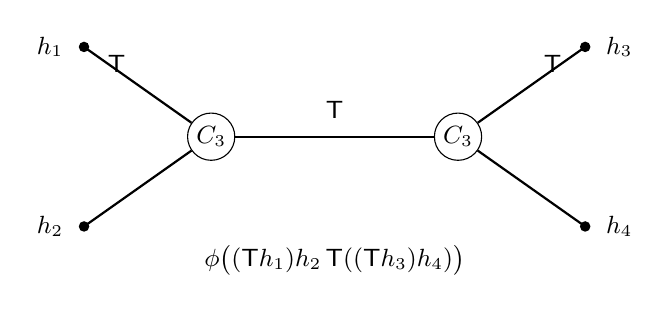
\begin{tikzpicture}[scale=.95,>=Latex,every node/.style={font=\small},
 junction/.style={circle,draw,fill=white,minimum size=6mm,inner sep=1pt}]
 \node[junction] (a) at (-1.65,0) {$C_3$};
 \node[junction] (b) at (1.65,0) {$C_3$};
 \coordinate (l1) at (-3.35,1.2);
 \coordinate (l2) at (-3.35,-1.2);
 \coordinate (l3) at (3.35,1.2);
 \coordinate (l4) at (3.35,-1.2);
 \draw[thick] (a)--(b) node[midway,above=3pt] {$\T$};
 \draw[thick] (a)--(l1) node[pos=.52,above left] {$\T$};
 \draw[thick] (a)--(l2);
 \draw[thick] (b)--(l3) node[pos=.52,above right] {$\T$};
 \draw[thick] (b)--(l4);
 \fill (l1) circle(2pt) node[left=4pt] {$h_1$};
 \fill (l2) circle(2pt) node[left=4pt] {$h_2$};
 \fill (l3) circle(2pt) node[right=4pt] {$h_3$};
 \fill (l4) circle(2pt) node[right=4pt] {$h_4$};
 \node at (0,-1.65)
 {$\phi\bigl((\T h_1)h_2\,\T((\T h_3)h_4)\bigr)$};
\end{tikzpicture}

\caption{A strict source with four original leaves. Each trivalent
vertex carries the symmetric product tensor. The middle edge has
a turn, so it is retained. A flagged leaf supplies $\T h_i$;
the other leaves supply $h_i$. Each vertex has one flagged
leaf. The labels $i$ remain independent when colors or crossings
are changed.}\label{st:tree-figure}
\end{figure}

For later estimates it is useful to record the exact outgoing
coupons. Root at a flagged leaf when one is present. A
nonroot junction gives
\begin{equation}\label{st:messages}
 Q_v=
 \begin{cases}
 \T\bigl(p_{i(v)}\prod_wQ_w\prod_lh_l\bigr),
       &\text{one flagged leaf},\\
 \T\bigl(\prod_wQ_w\prod_lh_l\bigr),
       &\text{no flagged leaf},
 \end{cases}
 \qquad p_i=\T h_i .
\end{equation}
The final scalar is $\phi(p_0\prod Q_w\prod h_l)$.
These are exact full-algebra identities, also for
$h_i=\T(R^{\eps_i}L_{j_i})$ at independent colors and signs.
The two outgoing types are respectively $L$ and $A$.
Commutativity and $\T^2=I$ in this calculation are not
claims that arbitrary physical turns or products can be
removed from the underlying tangle.

\begin{corollary}[Exposing any original leaf]\label{st:any-root}
Every original leaf of a strict closed tree with $H\ge3$
can be exposed as a closing character without changing
any other leaf. If its reduced edge parity is $\sigma$,
and $A$ is the product of the other branches at its
junction, then
\[
 Z_N=\phi((\T^\sigma h_j)A)
     =\phi(h_j\T^\sigma A)
     =\phi(p_j\T^{\sigma+1}A),\qquad p_j=\T h_j .
\]
The last factor is either an unturned product of at least
two $L/A$ branches, a decorated low module of the first
form in \eqref{st:messages}, or the turned output of an
unflagged product with at least two branches.
\end{corollary}
\begin{proof}
The pairing in \eqref{st:pairing} makes $\T$ self-adjoint:
$\phi((\T F)G)=\phi(F(\T G))$. This proves the identities.
If $\sigma=1$, the root leaf uses the only possible flag,
so all other branches are $L/A$ and
$\T^{\sigma+1}A=A$.
If $\sigma=0$ and another leaf at the junction is flagged,
$A=p_i\prod Q$ and $\T A$ is the decorated low module.
If there is no such flag, $\T A$ is the outgoing
unflagged product. The valence is at least three in
all cases. In particular an entirely unflagged
three-leaf tree is included.
\end{proof}
For a two-input product, two high Newton coordinates
vanish exactly: if $i,j>M$, then $i+j>d$ at both
parities. This finite observation is useful when the
last case of Corollary~\ref{st:any-root} has only
two inputs. It does not by itself bound a signed
character at the exposed root.

\section{The primitive polytope and its interior maximum}\label{st:variation}\label{nt:variational}
For a fixed strict expression let $P$ be the compact polytope
obtained by replacing all strict leaf and product inequalities
by their weak versions. Turns retain $y=1-x$, and closure
retains the complementary relation. Its relative interior is
the strict state set: a strict state exists, so none of the
listed proper inequalities is identically an equality.

\subsection{Integer coordinates and endpoints}
\begin{lemma}[Primitive coordinates]\label{st:lattice}
A closed tree with $H$ leaves has $K=2H-3$ free integer
coordinates after the forced closing product is removed.
Every remaining finite label has the form
\begin{equation}\label{st:offsets}
 r_w=NL_w(k/N)+\delta_w,\qquad k\in\ZZ^K,
\end{equation}
where $L_w$ is integral affine and $\delta_w$ is a fixed
integer. There is no residual congruence restriction.
Every strict real state is approached by admissible states
at all sufficiently large levels of both parities.
For an open tree the full dimension is $2H-1$ and its
fixed-output slice has dimension $2H-2$.
\end{lemma}
\begin{proof}
Keep a coordinate for every leaf output and every product
output. A unary turn simply replaces its input by $d-r$.
The closed tree has $H-2$ retained products, in addition
to its $H$ leaves. Its two root subtrees are disjoint,
so the closing relation can be solved for an output
coordinate in one subtree with coefficient $1$ or $-1$.
No identification of the two root coordinates has been
made. In particular, this procedure never creates $2r=d$.
This proves the dimension and primitivity assertions.
Replacing $d$ by $N-1$ gives \eqref{st:offsets}.

Round $d$ times the free coordinates of a strict state,
and reconstruct the eliminated coordinate exactly.
The errors in all labels are bounded for the fixed
expression. Every proper inequality has a positive
slack times $d$, so the rounded state is admissible
for all sufficiently large $N$. The strict leaf slack
also puts its labels below $M$, at either parity.
For a prescribed open output $r_N/d\to b$ in the actual
strict interval, choose strict states continuously
near $b$, fix that output first and round the other
coordinates. Such a continuous choice is obtained by
interpolating two nearby strict states with output
on either side of $b$.
\end{proof}

Define
\begin{align}
 J(t)&=\int_0^t\log(2\sin\pi u)\dd u,\qquad 0\le t\le1,
       \label{st:J}\\
 g(a)&=J(2a)-4J(a)
       =-2J(a)-2J(1/2-a),\label{st:g}\\
 m(x,y,z)&=J(x+y)+J(z)-J(x)-J(y)\notag\\
 &\hspace{11mm}-J(z-x)-J(z-y)-J(x+y-z).
       \label{st:m}
\end{align}
Here $J$ has its continuous endpoint values,
$J(1-t)=-J(t)$ and $J(1/2)=0$.
The complete action is the sum of one $g$ for each
original leaf and one $m$ for each retained product:
\begin{equation}\label{st:action}
 \A(y)=\sum_{\ell=1}^H g(a_\ell(y))
             +\sum_{v=1}^{H-2}m(x_v(y),y_v(y),z_v(y)).
\end{equation}
We write $\A_E$ when the expression $E$ must be specified.
For an open expression the sum contains all its products.

\begin{lemma}[Uniform factorial estimate]\label{lem:factorial-action}
Uniformly for $0\le r<N$,
\[
 \log S_r=NJ(r/N)+O(\log N).
\]
For a fixed tree, every nonzero complete state of scaled labels $\mathbf r/d$ has weight
\begin{equation}\label{st:weight-rate}
 \log w_N(\mathbf r)=N\A(\mathbf r/d)+O_E(\log N).
\end{equation}
\end{lemma}
\begin{proof}
Away from the endpoints, compare the sum of $\log(2\sin\pi u)$ with its integral on consecutive mesh cells. Near zero and one, subtract $\log u$ or $\log(1-u)$; the remaining function has bounded derivative, and the logarithmic part is controlled by factorials. The total discrepancy is $O(\log N)$, uniformly in the stopping index. Apply this estimate to \eqref{eq:positive-product} and \eqref{eq:complete-leaf}. The shifts between $r/N$ and $r/d$, and between $M/N$ and $1/2$, change $NJ$ by at most $O(\log N)$ because $J$ has modulus of continuity $O(\delta|\log\delta|)$. There are a fixed number of factors.
\end{proof}

\subsection{The atoms and their boundary derivative}
For $a+b+c=1$ set
\[
 V(a,b,c)=-\pi\{J(a)+J(b)+J(c)\}.
\]
This is a nonnegative function, zero on the boundary of
the angle simplex and positive in its interior.
Only these elementary properties and its derivatives
are used here. With $c=1-a-b$ its Hessian has entries
\[
 -\pi^2
 \begin{pmatrix}
  \cot\pi a+\cot\pi c&\cot\pi c\\
  \cot\pi c&\cot\pi b+\cot\pi c
 \end{pmatrix}.
\]
Both displayed diagonal sums are positive, and the
determinant is $\pi^4$, since
$\cot\pi a\cot\pi b+\cot\pi b\cot\pi c+
\cot\pi c\cot\pi a=1$. The Hessian is therefore negative
definite at a positive triple.

At a product put
\[
 p=z-x,\quad q_0=z-y,\quad r=x+y-z,\quad w=1-x-y.
\]
The subscript on $q_0$ distinguishes this angle from
the root of unity. Direct substitution gives
\begin{align}
 \pi g(a)&=2V(a,1/2-a,1/2),\label{st:leaf-atoms}\\
 \pi m(x,y,z)&=
 V(y,x,w)+V(p,q_0,2r+w)+V(p+q_0,r,r+w).
 \label{st:gate-atoms}
\end{align}
All three entries of each atom are nonnegative and sum
to one on the original gate support. Consequently the
whole action is concave on its shared-label polytope.

There are two different kinds of flat atom. At
$(0,a,1-a)$ with $0<a<1$, the directional derivative
toward a positive atom is $+\infty$:
$-J(t)=-t\log t+O(t)$ near zero.
At $(0,0,1)$ the singularities cancel. More explicitly,
along the segment with small entries $t\alpha,t\beta$,
\[
 V(t\alpha,t\beta,1-t(\alpha+\beta))
 =\pi t\{(\alpha+\beta)\log(\alpha+\beta)
                  -\alpha\log\alpha-\beta\log\beta\}
       +O(t^2).
\]
The derivative is finite. A positive atom also has a
finite derivative. Thus no atom contributes $-\infty$
along a segment toward a strict state.

\begin{lemma}[Endpoint descent]\label{st:barrier}
At every nonstrict point of a nonempty strict closed
polytope, or of an open fixed-output slice with output
in its strict interval, at least one atom in
\eqref{st:leaf-atoms}--\eqref{st:gate-atoms} is flat
but is not a vertex of its angle simplex.
\end{lemma}
\begin{proof}
First suppose a proper wire has value zero or one.
A turn replaces it by its complementary endpoint.
At a product with output zero both inputs are zero.
At a product with output one the inputs sum to one:
if both are interior, the first atom is $(y,x,0)$,
as required; otherwise one may descend to an endpoint
child. Repeating this descent in the finite tree
terminates at a leaf endpoint. A leaf of value zero
has atom $(0,1/2,1/2)$; a leaf cannot have value one.
The same argument applies to either child of the
deleted root: one descends inside that child, without
putting the removed flat gate back.

Suppose now that every wire is in $(0,1)$.
A leaf at its allowed upper endpoint $1/2$ gives
$(1/2,0,1/2)$. If every leaf is strict, a nonstrict
state must lie on a retained gate face.
When $w=0$, the first atom $(y,x,0)$ is nonvertex-flat.
When $r=0$, the third atom is $(z,0,1-z)$.
When $p=0$ and $q_0>0$, the second atom has one zero
entry and two positive entries; the case $q_0=0<p$
is symmetric. In the remaining intersection
$p=q_0=0$, one has $x=y=z\in(0,1)$ and the third
atom is $(0,x,1-x)$. This lists every gate boundary.

For a fixed-output slice the output itself is in
$(0,1)$, and the same descent applies to each proper
endpoint wire. The segment used below keeps that
output fixed. No boundary caused only by imposing
the output is included among these proper faces.
\end{proof}

\begin{theorem}[Unique strict optimizer]\label{st:positive-action}
Every strict closed expression has a unique maximizer
$y_*$ of its complete action. It is strict and its
Hessian in the primitive coordinates is negative
definite. The positive scalar satisfies the all-level
limit
\begin{equation}\label{st:positive-limit}
 \lim_{N\to\infty}\frac1N\log Z_N^0=F_0,\qquad
 F_0=\A(y_*)>0 .
\end{equation}
For an open expression of nonempty type, each output
$b$ in its strict interval has a unique strict
fixed-output maximizer. The profile
\[
 f_E(b)=\max_{\text{output }b}\A_E
\]
is real analytic and strictly concave on that interval.
It has a continuous extension to the closed feasible
output interval.
\end{theorem}
\begin{proof}
Compactness gives a maximizer. Join a nonstrict point
to a strict state in the same polytope. By
Lemma~\ref{st:barrier}, one atom contributes $+\infty$
to the one-sided derivative, and none contributes
$-\infty$. Hence the action increases and the point
cannot maximize.

At a strict product the gate Hessian is already
negative definite in $(x,y,z)$. Indeed the first
atom in \eqref{st:gate-atoms} detects
$(\delta x,\delta y)$; if those vanish, the second
detects $\delta z$. Its third atom is nonpositive
and cannot cancel either negative term.
The leaf Hessian is strictly negative since
\[
 g'(a)=2\log\cot\pi a,\qquad
 g''(a)=-\frac{4\pi}{\sin2\pi a}<0 .
\]
If all atom variations vanish, every leaf output
and retained product output is fixed. Turns then
fix their output wires, and the closing relation
fixes the eliminated coordinate. Thus the sum is
negative definite on the primitive tangent space.
This proves uniqueness by concavity.

For an open expression the same argument applies
including its output coordinate: its last product
detects that coordinate, or the expression is a
turned leaf and its leaf detects it. On a fixed-output
slice, the internal Hessian is therefore invertible.
The analytic implicit-function theorem gives a
real analytic maximizing state and profile.
The full negative Hessian has a negative Schur
complement in the output coordinate, so $f_E''<0$.
For the single-leaf case this is the displayed
formula and its reflection.

Continuity at a feasible endpoint is worth recording.
For any endpoint maximizing state, interpolate it
with an interior strict state. This supplies states
at every nearby interior output, and their actions
converge to the endpoint maximum. Conversely, every
sequence of maximizing states has a convergent
subsequence in the compact full polytope; its limit
is feasible at the endpoint. These two observations
prove continuity. They do not require finite support
at the exact endpoint for every parity.

There are at most $N^K$ positive states.
Equation~\eqref{st:weight-rate} gives the upper
limit in \eqref{st:positive-limit}. Primitive
rounding of $y_*$ gives a genuine positive summand
at every sufficiently large $N$ and the matching
lower limit. The strict leaf atoms are positive,
so $F_0>0$.
\end{proof}

\begin{lemma}[Gate curvature without leaf curvature]\label{st:gate-curvature}
For a closed strict tree with $H\ge3$, the sum of the
retained gate Hessians is itself negative definite
in the primitive coordinates.
\end{lemma}
\begin{proof}
Contract unary turn chains. Every wire in a nontrivial
root subtree appears at a retained product, either
as an input or as an output. If all gate variations
vanish, these wires have zero variation. The only
possible uncovered root subtree is a single leaf
with turns; its variation is fixed by the complementary
root relation and the other subtree. Both subtrees
can be single leaves only when $H=2$. The injectivity
and the strict gate Hessian proved above give the result.
\end{proof}

\section{Stationary boundary profiles and their constants}\label{st:profile-section}\label{nt:boundary}
The derivative of a fixed-output profile describes how the
maximum changes when the output moves. It is convenient to
record this derivative together with the output itself.
For a strict open output $b$, define
\begin{equation}\label{st:port}
 B=\cot\pi b,\qquad \kappa_E=e^{-f_E'(b)},\qquad
 X=\sqrt{\frac{1+B^2}{1+\kappa_E}},\qquad
 Y=\sqrt{\kappa_E}\,X .
\end{equation}
The square roots are positive. Thus
$X^2+Y^2-B^2=1$ and $f_E'(b)=2\log(X/Y)$.
We call $(B,X,Y)$ the stationary boundary parameters.
Their definitions are variational; no global geometric
realization is assumed.

\begin{lemma}[The stationary product]\label{st:port-product}
At a strict stationary product the two children and the
output have the same $X$. With child cotangents $B_1,B_2$,
\begin{equation}\label{st:port-product-equations}
 S=B_1+B_2>0,\qquad
 B_o=\frac{B_1B_2+X^2-1}{S},\qquad
 Y_o=\frac{Y_1Y_2}{S}.
\end{equation}
A turn sends $(B,X,Y)$ to $(-B,Y,X)$.
\end{lemma}
\begin{proof}
At inputs $x,y$ and output $z$, stationarity gives
$f_1'(x)=-m_x$, $f_2'(y)=-m_y$ and $f_o'(z)=m_z$.
Differentiating \eqref{st:m} yields
\begin{align*}
 e^{m_x}&=\frac{\sin\pi(x+y)\sin\pi(z-x)}
                  {\sin\pi x\sin\pi(x+y-z)},\\
 e^{m_y}&=\frac{\sin\pi(x+y)\sin\pi(z-y)}
                  {\sin\pi y\sin\pi(x+y-z)},\\
 e^{-m_z}&=\frac{\sin\pi(z-x)\sin\pi(z-y)}
                  {\sin\pi z\sin\pi(x+y-z)}.
\end{align*}
Set $D=1-B_1B_2+B_o(B_1+B_2)$. The identities
\[
 S=\frac{\sin\pi(x+y)}{\sin\pi x\sin\pi y}>0,\qquad
 D=\frac{\sin\pi(x+y-z)}
          {\sin\pi x\sin\pi y\sin\pi z}>0
\]
and \eqref{st:port} give
\[
 X_1^2=X_2^2=X_o^2=D,\quad
 Y_1^2=S(B_1-B_o),\quad Y_2^2=S(B_2-B_o),\quad
 Y_o^2=(B_1-B_o)(B_2-B_o).
\]
Taking positive roots proves the product formulas.
For a turn $f_{\T E}(b)=f_E(1-b)$, so its derivative
changes sign and its cotangent changes sign. This
proves the last assertion.
\end{proof}

\begin{proposition}[Parameters of the three types]\label{st:port-types}
On their actual strict output intervals the parameters satisfy
\begin{equation}\label{st:parameter-table}
 \begin{array}{c|c}
 L&(B,X,Y)=(B,B,1),\quad B>0,\\
 H&(B,X,Y)=(-Y,1,Y),\quad Y>0,\\
 A&-Y<B<X.
 \end{array}
\end{equation}
Consequently there are constants $c_E$ such that
\begin{equation}\label{st:rigid-profiles}
 f_E(b)=g(b)+c_E\quad(E:L),\qquad
 f_E(b)=g(1-b)+c_E\quad(E:H).
\end{equation}
\end{proposition}
\begin{proof}
For a leaf, $g'=2\log\cot\pi b$ gives $(B,B,1)$.
The turn formula exchanges the first two rows and
preserves the inequality in the third.
Consider the products giving type $A$, whose children
have type $L$ or $A$.
If the common $X<1$, put $h_0=\sqrt{1-X^2}$ and write
\[
 B_i=h_0\cot\alpha_i,\qquad
 Y_i=h_0\csc\alpha_i,\qquad 0<\alpha_i<\pi.
\]
The low type has $\alpha_i=\arccos X$ and the
unrestricted type has $\alpha_i>\arccos X$.
The positivity of $S$ gives $\alpha_1+\alpha_2<\pi$,
and \eqref{st:port-product-equations} adds these angles.
Therefore $B_o<X$ and
$B_o+Y_o=h_0\cot((\alpha_1+\alpha_2)/2)>0$.
If $X\ge1$, each child has
$\sqrt{X^2-1}<B_i\le X$, with equality at the
upper bound allowed for type $L$.
In particular $B_o>0$, and
\[
 (X-B_1)(X-B_2)<1
\]
implies $B_o<X$ by \eqref{st:port-product-equations}.
The strict inequality holds also at $X=1$, since
each $B_i>0$.

A product giving type $H$ has one high child, with
parameters $(-u,1,u)$. Hence the common $X=1$.
Its other child, of type $L$ or $A$, has parameters
$(b,1,b)$ with $b>0$. Strictness says $b-u>0$,
and the output is
\[
 \left(-\frac{ub}{b-u},1,\frac{ub}{b-u}\right).
\]
This proves all cases of the table.
Finally the first two rows determine $f_E'$ as
the derivative of $g(b)$ or $g(1-b)$ on the
connected strict interval, giving \eqref{st:rigid-profiles}.
Their constants are computed next, without a choice
of additive normalization.
\end{proof}

\subsection{The intrinsic satellite action}
No product has type $L$. A product of type $H$ has
exactly one high child. Starting at an $L$ or $H$
output, follow turns and the unique high child of
each product. This path terminates at a unique
original leaf, the \emph{distinguished leaf}.
The other children on the path are called its
satellites, and have type $L$ or $A$.
Between successive high products the number of turns
is even. Thus the full algebra also gives
\begin{equation}\label{st:spine-source}
 E_H=(\T h_*)\prod_{j=1}^m Q_j,\qquad
 E_L=\T\left((\T h_*)\prod_{j=1}^m Q_j\right),
\end{equation}
after associating the inherited products. This
identity retains the actual polynomials; its
stationary profile is simpler than the polynomial.

For a satellite $Q$ define
\begin{equation}\label{st:Omega}
 \Omega_Q=\max_{0\le a\le1/2}\{g(a)+f_Q(a)\}.
\end{equation}
The maximum is the complete action of the literal
strict closure $C(h\,\T Q)$. The strict type of
$Q$ is $L$ or $A$, so Theorem~\ref{st:positive-action}
gives a unique strict maximizer $\beta_Q$.
Its equation is
$g'(\beta_Q)+f_Q'(\beta_Q)=0$.
Consequently the satellite has parameters
\begin{equation}\label{st:satellite-parameters}
 (B_Q,X_Q,Y_Q)=(b_Q,1,b_Q),\qquad
 b_Q=\cot\pi\beta_Q>0 .
\end{equation}
For type $L$, $\beta_Q=1/4$ and $b_Q=1$;
for type $A$, the strict inequality $B_Q<X_Q$
gives $1/4<\beta_Q<1/2$ and $0<b_Q<1$.

\begin{theorem}[Harmonic response and absolute profiles]\label{st:profiles}
For the spine \eqref{st:spine-source}, let $u_0$
be the cotangent of its distinguished original leaf.
Let $v$ be the final high output's $Y$, equivalently
the final low output's $X$. At its stationary state,
\begin{equation}\label{st:harmonic}
 \frac1{u_0}=\frac1v+\sum_{j=1}^m\frac1{b_{Q_j}},
 \qquad
 c_E=\sum_{j=1}^m\Omega_{Q_j}.
\end{equation}
In particular \eqref{st:rigid-profiles} holds with
exactly this constant. The parameters $b_{Q_j}$
depend only on the corresponding satellites.
\end{theorem}
\begin{proof}
Every high product has common $X=1$, so its satellite
is at the unique state \eqref{st:satellite-parameters}.
With high input $(-u,1,u)$ and output $(-v,1,v)$,
\eqref{st:port-product-equations} gives
\begin{equation}\label{st:one-response}
 v=\frac{ub}{b-u},\qquad
 0<u<b,\qquad \frac1u=\frac1v+\frac1b .
\end{equation}
Iteration proves the first formula. Conversely every
$v,b>0$ gives the strict branch $0<u<b$; no sign
has been lost by squaring the stationary equations.

It remains to fix the constant. Suppose the incoming
high profile is $g(1-x)+c$. Send the outgoing high
label $z$ to one. Then
$v=-\cot\pi z\to+\infty$, $u\to b$ and
$x\to1-\beta_Q$. The last gate approaches
$x+\beta_Q=z=1$. Its continuous action is zero:
in \eqref{st:m} use $J(1-\beta_Q)=-J(\beta_Q)$,
or note that all three atoms in
\eqref{st:gate-atoms} are flat.
Continuity of profiles, proved in
Theorem~\ref{st:positive-action}, gives
\[
 c_{\rm out}=c+g(\beta_Q)+f_Q(\beta_Q)=c+\Omega_Q.
\]
Turns preserve the constant and the bare leaf has
constant zero. This proves the second formula.
\end{proof}
For a low satellite, $\Omega_Q=2G_0+c_Q$ where
$G_0=g(1/4)$. The formula is an identity of optimized
actions. For example at $N=3$ the complete source has
$h=10-z$ and $\T h=z^2-1$; their product is
$10z^2-2z-8$ in
$\CC[z]/((z-1)^2(z+2))$. It is not a scalar
multiple of $\T h$: the value ratio at $-2$ is
$12$, whereas the normal ratio at $1$ is $9$.
Thus the constant profile does not suppress normal
data of the source.

\subsection{Unrestricted components and their effective range}
Replace each maximal low subtree by its profile
$g+c_i$. A remaining type-$A$ subtree has syntax
\begin{equation}\label{st:skeleton}
 A::=LL\mid\T A\mid AA\mid LA\mid AL,
\end{equation}
where $L$ here is an effective profile, not a
replacement quantum leaf. The definition of the
maximum immediately gives
\begin{equation}\label{st:constant-skeleton}
 f_A(z)=f_{A^{\rm skel}}(z)+\sum_i c_i.
\end{equation}
At an unflagged junction directed toward a parent,
the outgoing expression is $Q=\T A$ with $A=FG$
an unturned product and both children of type $L$
or $A$. Its intrinsic action is
\[
 \Omega_Q=\max_{0\le a\le1/2}
                 \{g(a)+f_A(1-a)\}.
\]
This is the action of the strict closure $C(hA)$.

\begin{theorem}[The intrinsic probe range]\label{st:probe}
At this closing maximum the unturned output has
\begin{equation}\label{st:probe-port}
 (B_A,X_A,Y_A)=(-x,x,1),\qquad \frac12\le x<1.
\end{equation}
Every effective leaf in \eqref{st:skeleton},
including the closing probe, has cotangent in
$[1/2,1)$. Equality at $1/2$ occurs only when
the entire effective closure consists of three
leaves. In every other case all these cotangents
are strictly between $1/2$ and one.

The absolute identities are
\begin{equation}\label{st:probe-constant}
 \Omega_Q=F_{\rm probe}(A^{\rm skel})+\sum_i c_i,
 \qquad F_0=\sum_j\Omega_{Q_j}
\end{equation}
for a whole reduced tree rooted at a flagged leaf,
with satellites $Q_j$ at that root.
\end{theorem}
\begin{proof}
The root condition says that the two output labels
are complementary and their profile derivatives
agree. Hence their triples are $(B,X,Y)$ and
$(-B,X,Y)$. The bare probe has $(x,x,1)$,
so \eqref{st:probe-port} holds initially with
$0<x<1$, the strict upper bound coming from
$-Y_A<B_A$.
At the last product use the identities in the
proof of Lemma~\ref{st:port-product}:
\[
 1=Y_A^2=(B_F-B_A)(B_G-B_A)
             \le(X_A-B_A)^2=4x^2 .
\]
Both factors are positive because output labels
strictly exceed the inputs. This proves $x\ge1/2$.

At the root product every child has common $X=x<1$.
Its cotangent satisfies $B_i\le X$ and, by
$B_1+B_2>0$, also $B_i>-X$.
If it is type $A$, both inequalities are strict,
so $Y_i^2=1+B_i^2-X^2<1$.
Turns exchange $X,Y$. The same argument propagates
the strict bounds $X,Y<1$ through every proper
type-$A$ descendant.
For a low child $(X,X,1)$ and another child
$(B,X,Y)$, the output bound $Y_o\le1$ implies
\begin{equation}\label{st:effective-bound}
 1+B^2-X^2\le(B+X)^2,\qquad
 1\le2X(B+X)\le4X^2.
\end{equation}
The last inequality is strict for an unrestricted
neighbor. For two low children at a proper
descendant, the first is strict because $Y_o<1$.
Thus equality is possible only at the root
product with two effective low children. It
gives the three-leaf closure and $x=1/2$ at
all three leaves. This proves the range.

The first identity in \eqref{st:probe-constant}
is \eqref{st:constant-skeleton} inside the same
maximum. For the second, write the original
root source as $\phi((\T h_0)\prod Q_j)$.
The associated open high profile is
$g(1-z)+\sum_j\Omega_{Q_j}$ by
Theorem~\ref{st:profiles}. At the closing output
$z=1$ the deleted last gate has coefficient
one and $g(0)=0$. Profile continuity identifies
its endpoint maximum with precisely the original
closed action, proving the formula.
\end{proof}

One boundary case in later coefficient estimates can
be read directly from these parameters. If the last
product is $A=LF$ with $F$ unrestricted, then
\[
 B_F=\frac1{2x}-x,\qquad Y_F=\frac1{2x},\qquad
 f_F'=2\log(2x^2),\quad f_A'=2\log x .
\]
For $1/2\le x\le2/3$ both slopes lie in
$[-2\log2,0]$. This is an exact closed parameter
range; it does not assert an estimate for the
signed source. Such estimates require its actual
coefficient arrays.

\begin{corollary}[The action budget at any exposed leaf]\label{st:root-budget}
Use Corollary~\ref{st:any-root}, with root edge parity
$\sigma$ and remaining product $A$.
If $\sigma=1$, every branch of $A$ has type $L$ or
$A$ and the original complete action is
$F_0=\sum_Q\Omega_Q$, summed over those branches.
If $\sigma=0$, then $Q=\T A$ has type $L$ or $A$
and $\Omega_Q=F_0$.
\end{corollary}
\begin{proof}
For $\sigma=1$, this is the last identity of
\eqref{st:probe-constant} at the exposed flagged
root. For $\sigma=0$, the original positive closure
is $C(hA)$, whose action is exactly
$\max_a\{g(a)+f_A(1-a)\}=\Omega_{\T A}$.
This includes the decorated case in which $A$
has one high child and $\T A$ is low.
Only the finite source is rerooted; the variational
maximum and every physical leaf are unchanged.
\end{proof}

\section{The quarter bound at the original closed maximum}
\begin{theorem}[All original leaves are at or above quarter]\label{st:quarter}
At the unique complete maximum of any strict closed
expression, every stationary boundary triple satisfies $X,Y\le1$.
Every original leaf label therefore satisfies
\begin{equation}\label{st:quarter-bound}
 \frac14\le a_\ell(y_*)<\frac12 .
\end{equation}
Along an $L/H$ spine with $m$ satellites, its
distinguished original leaf additionally satisfies
$\cot(\pi a_*)\le1/(m+1)$.
\end{theorem}
\begin{proof}
At the complementary root the two triples have
opposite $B$ and equal $X,Y$. For type $AA$ the
inequalities give $|B|<\min(X,Y)$.
Together with $X^2+Y^2-B^2=1$ this gives
$X,Y<1$. For type $AL$, the low side is
$(x,x,1)$ and the unrestricted inequality
$-1<-x$ gives $x<1$.
For type $AH$, the high side has $X=1$,
and the unrestricted side gives $Y<1$.
For type $LH$, the two explicit forms force
$X=Y=1$. These exhaust the strict closing pairs.

Descend through a product. The common $X$ is
already at most one. Every child type satisfies
$B_i\le X$, and $B_1+B_2>0$ implies
$B_i>-B_j\ge-X$. Thus
$Y_i^2=1+B_i^2-X^2\le1$.
A turn exchanges the same two bounds.
At a leaf, $X=\cot\pi a>0$, proving
\eqref{st:quarter-bound}. Finally, in
\eqref{st:harmonic} one has $v\le1$ and
$b_{Q_j}\le1$, so $1/u_0\ge m+1$.
\end{proof}
The lower endpoint is attained. In
$C(h\,\T(h^s))$, the inner $s$ original leaves
have $X=1$ and hence label $1/4$.
Indeed their product has at $X=1$ the parameters
$B=Y=1/s$, its turn has $(-1/s,1/s,1)$, and
the closing leaf has cotangent $1/s$.
Thus strictness of every angle state does not force
its original leaf labels to lie strictly above one quarter.

\section{The completed-root subclass}\label{nt:completed}
The preceding results allow every strict ordered expression. The
following narrower recursive construction gives a stronger two-sided
bound at each original leaf.

\begin{definition}[Completed expressions]\label{def:grammar}
Start with the stack $hh$. One may turn a constructed box, stack two
constructed boxes, or attach a single elementary piece on either side.
Equivalently,
\[
 E::=hh\mid\Turn(E)\mid E_1E_2\mid hE\mid Eh.
\]
A closed expression is $C(FG)$ with both $F$ and $G$ completed.
The word ``completed'' specifies this rule; it has no metric meaning.
\end{definition}

\begin{lemma}[Strict feasibility]\label{lem:strict-feasible}
Every completed expression has a strict state at every output $b\in(0,1)$. Every completed/completed cylindrical closure has a strict reduced state.
\end{lemma}
\begin{proof}
For $hh$, choose equal leaves $a\in(b/2,\min(b,1/2))$. For a completed product choose its two outputs in the same interval and use induction in each child. For $hE$ or $Eh$, use that number for the bare leaf and for the completed child's output. A turn uses the child's strict state at $1-b$. At the closing product prescribe $1/2,1/2$ and remove its forced gate. All remaining inequalities are strict.
\end{proof}

By Lemma~\ref{st:types}, every completed expression has unrestricted
type $A$. The two conclusions below record the specialization used in
the completed-root applications. Write $Z_{F,G,N}=Z_N^0$ for the
complete scalar of $C(FG)$.

\begin{proposition}[Completed-root optimizer]\label{prop:strict-maximum}
After deleting the forced closing gate, every completed/completed
closure has a unique strict maximizer. Its Hessian on the primitive
coordinates is negative definite. The fixed-output profile $f_E(b)$
is real analytic on $0<b<1$ for every completed expression.
\end{proposition}
\begin{proof}
Lemma~\ref{lem:strict-feasible} supplies the strict state and full
output interval. Apply Theorem~\ref{st:positive-action}.
\end{proof}

\begin{corollary}[Completed-root positive-source limit]\label{cor:complete-limit}
For the positive complete scalar of $C(FG)$,
\[
 \lim_{N\to\infty}\frac1N\log Z_{F,G,N}
       =\max\mathcal A_{C(FG)}.
\]
\end{corollary}
\begin{proof}
This is the positive limit of Theorem~\ref{st:positive-action}
on the same original wire polytope, using its primitive lattice
approximation at every sufficiently large level of either parity.
\end{proof}

The stationary triples are exactly those of \eqref{st:port};
their product and turn rules are Lemma~\ref{st:port-product}.
The next argument strengthens the quarter bound on this subclass.

\begin{lemma}[Bounds on the boundary parameters]\label{lem:port-bounds}
The boundary parameters of every completed box satisfy $-Y<B<X$. In a completed/completed closure every completed descendant has $0<X,Y<1$, and every leaf satisfies
\begin{equation}\label{eq:leaf-window}
 \frac12<X_\ell=\cot\pi a_\ell<1,
 \qquad \frac14<a_\ell<\frac{\arctan2}{\pi}.
\end{equation}
\end{lemma}
\begin{proof}
The base $hh$ has $B=X-1/(2X)$ and $Y=1/(2X)$. Turns preserve the claimed inequality. For a single attachment, \eqref{st:port-product-equations} becomes
\[
 B_o=X-\frac1{X+B},\qquad Y_o=\frac{Y}{X+B}.
\]
For $X\ge1$, the child inequality forces $B>\sqrt{X^2-1}$ and the result follows. For $X<1$, let $h_0=\sqrt{1-X^2}$ and $\alpha=\arccos X$. Express a child as $(B,Y)=(h_0\cot\beta,h_0\csc\beta)$. A bare leaf has $\beta=\alpha$, a completed child has $\beta>\alpha$, and product adds the angles, with their sum below $\pi$. This proves the strict upper bound and the lower bound $B_o+Y_o=h_0\cot((\beta_1+\beta_2)/2)>0$. It also proves the completed/completed step when $X<1$. When $X\ge1$, both completed children satisfy $\sqrt{X^2-1}<B_i<X$. Hence $0<X-B_i<X-\sqrt{X^2-1}\le1$, so $(X-B_1)(X-B_2)<1$. Formula~\eqref{st:port-product-equations} then gives $B_o<X$, while $B_o>0$ proves the lower bound.

At closure the boundary triples of the two boxes are $(B,X,Y)$ and $(-B,X,Y)$. Applying both inequalities gives $|B|<\min(X,Y)$; the hyperboloid relation implies $X,Y<1$. In the angle chart, parent $Y<1$ puts the sum of child angles below $\pi-\alpha$, while each child angle is at least $\alpha$. Every completed child therefore has $Y<1$, and turns exchange the bounds. Finally, at a single attachment $Y_o<1$ gives
$1<2X(X+B)<4X^2$. At an $hh$ base it gives $1/(2X)<1$. Thus every leaf has $X>1/2$, proving \eqref{eq:leaf-window}.
\end{proof}

For a fixed tree the inequalities give a compact neighborhood of every selected leaf inside $(1/4,1/2)$. This supplies a compact interior interval for later complex source estimates. It is not a uniform bound over an unbounded family of trees.


\section{Reproduction and further uses}\label{nt:reproduction}
The accompanying runner executes both retained checkers with one command
from the repository root:
\begin{verbatim}
python3 papers/newton-calculus/check.py --output /tmp/newton-check
\end{verbatim}
The two checkers retain their distinct purposes.
The Newton checker compares physical matrix turns and cylindrical
traces with the displayed finite formulas in exact finite fields;
it includes the colored-circle coefficients and repeated-root
polynomial reduction. The support-and-profile checker enumerates
integer supports, checks different parenthesizations of multiple
products, and verifies rational instances of the stationary product
and harmonic identities. These finite tests detect coefficient,
indexing, phase and normalization errors. The all-level algebra,
interior maximum and limiting statements are proved in the text.

The positive-source limit uses a uniform factorial estimate, a
polynomial number of states and a positive summand approaching the
strict maximum at every sufficiently large level. Introducing retained
half twists or performing the fillings gives complex terms. The
resulting invariant requires separate bounds on all complementary
terms and a noncancellation argument. Likewise, stationary boundary
parameters are variational data; their global marked geometric
realization is not inferred here.

The polynomial relation in the finite calculation is the complete
one, $P_N$. Changing the main meridian changes that relation and some
turn factors. Those deformed identities require a separate calculation.

\begin{thebibliography}{9}
\bibitem{Finite}\emph{Finite spectral evaluation and uniform filling bounds}.
Companion paper, \href{https://sashakolpakov.github.io/murakamis_dream/papers/filling-bounds.pdf}{repository edition}.
\bibitem{Kashaev1995} R. M. Kashaev,
A link invariant from quantum dilogarithm,
\emph{Modern Physics Letters A} \textbf{10} (1995), 1409--1418.
\href{https://arxiv.org/abs/q-alg/9504020}{arXiv:q-alg/9504020}.
\bibitem{KauffmanLambropoulou} L. H. Kauffman and S. Lambropoulou,
On the classification of rational tangles,
\emph{Advances in Applied Mathematics} \textbf{33} (2004), 199--237.
\href{https://arxiv.org/abs/math/0311499}{arXiv:math/0311499}.
\bibitem{FuterGueritaud} D. Futer and F. Gu\'eritaud,
From angled triangulations to hyperbolic structures,
\emph{Contemporary Mathematics} \textbf{541} (2011), 159--182.
\href{https://arxiv.org/abs/1004.0440}{arXiv:1004.0440}.
\end{thebibliography}
\end{document}

